% Options for packages loaded elsewhere
\PassOptionsToPackage{unicode}{hyperref}
\PassOptionsToPackage{hyphens}{url}
%
\documentclass[
]{article}
\usepackage{amsmath,amssymb}
\usepackage{iftex}
\ifPDFTeX
  \usepackage[T1]{fontenc}
  \usepackage[utf8]{inputenc}
  \usepackage{textcomp} % provide euro and other symbols
\else % if luatex or xetex
  \usepackage{unicode-math} % this also loads fontspec
  \defaultfontfeatures{Scale=MatchLowercase}
  \defaultfontfeatures[\rmfamily]{Ligatures=TeX,Scale=1}
\fi
\usepackage{lmodern}
\ifPDFTeX\else
  % xetex/luatex font selection
\fi
% Use upquote if available, for straight quotes in verbatim environments
\IfFileExists{upquote.sty}{\usepackage{upquote}}{}
\IfFileExists{microtype.sty}{% use microtype if available
  \usepackage[]{microtype}
  \UseMicrotypeSet[protrusion]{basicmath} % disable protrusion for tt fonts
}{}
\makeatletter
\@ifundefined{KOMAClassName}{% if non-KOMA class
  \IfFileExists{parskip.sty}{%
    \usepackage{parskip}
  }{% else
    \setlength{\parindent}{0pt}
    \setlength{\parskip}{6pt plus 2pt minus 1pt}}
}{% if KOMA class
  \KOMAoptions{parskip=half}}
\makeatother
\usepackage{xcolor}
\usepackage[margin=1in]{geometry}
\usepackage{color}
\usepackage{fancyvrb}
\newcommand{\VerbBar}{|}
\newcommand{\VERB}{\Verb[commandchars=\\\{\}]}
\DefineVerbatimEnvironment{Highlighting}{Verbatim}{commandchars=\\\{\}}
% Add ',fontsize=\small' for more characters per line
\usepackage{framed}
\definecolor{shadecolor}{RGB}{248,248,248}
\newenvironment{Shaded}{\begin{snugshade}}{\end{snugshade}}
\newcommand{\AlertTok}[1]{\textcolor[rgb]{0.94,0.16,0.16}{#1}}
\newcommand{\AnnotationTok}[1]{\textcolor[rgb]{0.56,0.35,0.01}{\textbf{\textit{#1}}}}
\newcommand{\AttributeTok}[1]{\textcolor[rgb]{0.13,0.29,0.53}{#1}}
\newcommand{\BaseNTok}[1]{\textcolor[rgb]{0.00,0.00,0.81}{#1}}
\newcommand{\BuiltInTok}[1]{#1}
\newcommand{\CharTok}[1]{\textcolor[rgb]{0.31,0.60,0.02}{#1}}
\newcommand{\CommentTok}[1]{\textcolor[rgb]{0.56,0.35,0.01}{\textit{#1}}}
\newcommand{\CommentVarTok}[1]{\textcolor[rgb]{0.56,0.35,0.01}{\textbf{\textit{#1}}}}
\newcommand{\ConstantTok}[1]{\textcolor[rgb]{0.56,0.35,0.01}{#1}}
\newcommand{\ControlFlowTok}[1]{\textcolor[rgb]{0.13,0.29,0.53}{\textbf{#1}}}
\newcommand{\DataTypeTok}[1]{\textcolor[rgb]{0.13,0.29,0.53}{#1}}
\newcommand{\DecValTok}[1]{\textcolor[rgb]{0.00,0.00,0.81}{#1}}
\newcommand{\DocumentationTok}[1]{\textcolor[rgb]{0.56,0.35,0.01}{\textbf{\textit{#1}}}}
\newcommand{\ErrorTok}[1]{\textcolor[rgb]{0.64,0.00,0.00}{\textbf{#1}}}
\newcommand{\ExtensionTok}[1]{#1}
\newcommand{\FloatTok}[1]{\textcolor[rgb]{0.00,0.00,0.81}{#1}}
\newcommand{\FunctionTok}[1]{\textcolor[rgb]{0.13,0.29,0.53}{\textbf{#1}}}
\newcommand{\ImportTok}[1]{#1}
\newcommand{\InformationTok}[1]{\textcolor[rgb]{0.56,0.35,0.01}{\textbf{\textit{#1}}}}
\newcommand{\KeywordTok}[1]{\textcolor[rgb]{0.13,0.29,0.53}{\textbf{#1}}}
\newcommand{\NormalTok}[1]{#1}
\newcommand{\OperatorTok}[1]{\textcolor[rgb]{0.81,0.36,0.00}{\textbf{#1}}}
\newcommand{\OtherTok}[1]{\textcolor[rgb]{0.56,0.35,0.01}{#1}}
\newcommand{\PreprocessorTok}[1]{\textcolor[rgb]{0.56,0.35,0.01}{\textit{#1}}}
\newcommand{\RegionMarkerTok}[1]{#1}
\newcommand{\SpecialCharTok}[1]{\textcolor[rgb]{0.81,0.36,0.00}{\textbf{#1}}}
\newcommand{\SpecialStringTok}[1]{\textcolor[rgb]{0.31,0.60,0.02}{#1}}
\newcommand{\StringTok}[1]{\textcolor[rgb]{0.31,0.60,0.02}{#1}}
\newcommand{\VariableTok}[1]{\textcolor[rgb]{0.00,0.00,0.00}{#1}}
\newcommand{\VerbatimStringTok}[1]{\textcolor[rgb]{0.31,0.60,0.02}{#1}}
\newcommand{\WarningTok}[1]{\textcolor[rgb]{0.56,0.35,0.01}{\textbf{\textit{#1}}}}
\usepackage{graphicx}
\makeatletter
\def\maxwidth{\ifdim\Gin@nat@width>\linewidth\linewidth\else\Gin@nat@width\fi}
\def\maxheight{\ifdim\Gin@nat@height>\textheight\textheight\else\Gin@nat@height\fi}
\makeatother
% Scale images if necessary, so that they will not overflow the page
% margins by default, and it is still possible to overwrite the defaults
% using explicit options in \includegraphics[width, height, ...]{}
\setkeys{Gin}{width=\maxwidth,height=\maxheight,keepaspectratio}
% Set default figure placement to htbp
\makeatletter
\def\fps@figure{htbp}
\makeatother
\setlength{\emergencystretch}{3em} % prevent overfull lines
\providecommand{\tightlist}{%
  \setlength{\itemsep}{0pt}\setlength{\parskip}{0pt}}
\setcounter{secnumdepth}{-\maxdimen} % remove section numbering
\ifLuaTeX
  \usepackage{selnolig}  % disable illegal ligatures
\fi
\usepackage{bookmark}
\IfFileExists{xurl.sty}{\usepackage{xurl}}{} % add URL line breaks if available
\urlstyle{same}
\hypersetup{
  pdftitle={Bellabeat\_project},
  pdfauthor={Jorge Ramírez},
  hidelinks,
  pdfcreator={LaTeX via pandoc}}

\title{Bellabeat\_project}
\author{Jorge Ramírez}
\date{2024-08-26}

\begin{document}
\maketitle

{
\setcounter{tocdepth}{3}
\tableofcontents
}
\subsection{Proyecto de Análisis para Bellabeat (Curso Análisis de Datos
de
Google)}\label{proyecto-de-anuxe1lisis-para-bellabeat-curso-anuxe1lisis-de-datos-de-google}

\begin{figure}
\centering
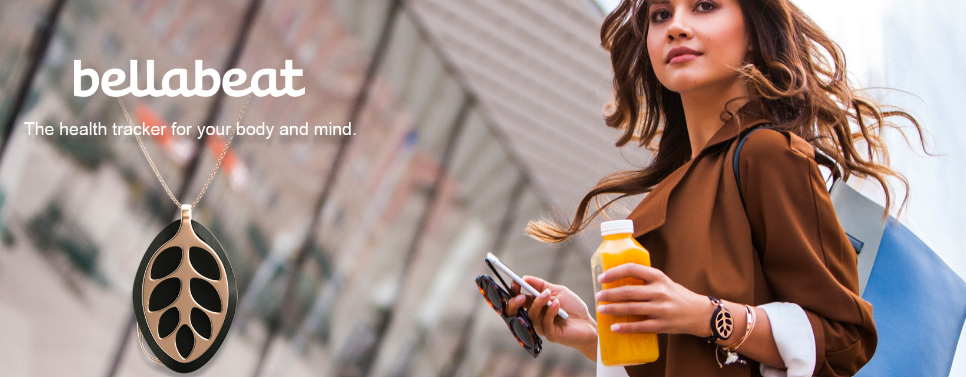
\includegraphics{images/Bellabeat_head.png}
\caption{Imagen propiedad de Bellabeat}
\end{figure}

Bellabeat representa más que una marca; Es un testimonio del
empoderamiento de las mujeres a través de la tecnología. Para mí, se
trata de crear un futuro en el que el bienestar se integre a la
perfección en todos los aspectos de nuestras vidas.

\begin{figure}
\centering

\includegraphics{images/What_we_do.png}
\caption{Productos que vendemos}
\end{figure}

Somos una marca, a la vanguardia de la tecnología dedicada activamente a
la salud y multipremiada.

\section{1 -- Tarea Empresarial:}\label{tarea-empresarial}

Concentrarnos en uno de los productos de Bellabeat y analizar los datos
de los dispositivos inteligentes para conocer el uso que hacen los
consumidores de sus dispositivos inteligentes. Saber cómo usan los
consumidores los dispositivos inteligentes que no son de Bellabeat, para
nos recomendó usar entre una de las fuentes datos de una investigación
realizada por Fitbit.

\url{https://www.kaggle.com/arashnic/fitbit}

\section{Metadatos:}\label{metadatos}

Este conjunto de datos fue generado personas que respondieron a través
de encuesta distribuida por Amazon Mechanical Turk. Fecha: entre el
03.12.2016 y el 05.12.2016. Muestreo: Treinta usuarios elegibles de
Fitbit dieron su consentimiento para el envío de datos de seguimiento
personal. Datos: a nivel de minuto para la actividad física, la
frecuencia cardíaca y el monitoreo del sueño. Los informes individuales
se pueden analizar por ID de sesión de exportación (columna A) o marca
de tiempo (columna B). La variación entre los resultados representa el
uso de diferentes tipos de monitores Fitbit y los
comportamientos/preferencias de seguimiento individuales.

\includegraphics{images/Fitbit.png} \# Limitaciones de nuestro dataset:
Solo se observa a 30 personas, desconocemos las edades, el sexo y la
ubicación geográfica, la ventana de observación son solo 2 meses. Los
datos Si son Confiables y Originales, No son Integrales, No son
actuales.

\section{Inicio del trabajo:}\label{inicio-del-trabajo}

\begin{verbatim}
## Warning: package 'tidyverse' was built under R version 4.4.1
\end{verbatim}

\begin{verbatim}
## Warning: package 'ggplot2' was built under R version 4.4.1
\end{verbatim}

\begin{verbatim}
## Warning: package 'tibble' was built under R version 4.4.1
\end{verbatim}

\begin{verbatim}
## Warning: package 'tidyr' was built under R version 4.4.1
\end{verbatim}

\begin{verbatim}
## Warning: package 'readr' was built under R version 4.4.1
\end{verbatim}

\begin{verbatim}
## Warning: package 'purrr' was built under R version 4.4.1
\end{verbatim}

\begin{verbatim}
## Warning: package 'dplyr' was built under R version 4.4.1
\end{verbatim}

\begin{verbatim}
## Warning: package 'stringr' was built under R version 4.4.1
\end{verbatim}

\begin{verbatim}
## Warning: package 'forcats' was built under R version 4.4.1
\end{verbatim}

\begin{verbatim}
## Warning: package 'lubridate' was built under R version 4.4.1
\end{verbatim}

\begin{verbatim}
## -- Attaching core tidyverse packages ------------------------ tidyverse 2.0.0 --
## v dplyr     1.1.4     v readr     2.1.5
## v forcats   1.0.0     v stringr   1.5.1
## v ggplot2   3.5.1     v tibble    3.2.1
## v lubridate 1.9.3     v tidyr     1.3.1
## v purrr     1.0.2     
## -- Conflicts ------------------------------------------ tidyverse_conflicts() --
## x dplyr::filter() masks stats::filter()
## x dplyr::lag()    masks stats::lag()
## i Use the conflicted package (<http://conflicted.r-lib.org/>) to force all conflicts to become errors
\end{verbatim}

\begin{verbatim}
## Warning: package 'patchwork' was built under R version 4.4.1
\end{verbatim}

\begin{verbatim}
## Warning: package 'ggthemes' was built under R version 4.4.1
\end{verbatim}

\section{Exploración Extraccion y Limpieza de Set de Datos de
Fitbit.}\label{exploraciuxf3n-extraccion-y-limpieza-de-set-de-datos-de-fitbit.}

\begin{Shaded}
\begin{Highlighting}[]
\CommentTok{\# Obtener la lista de archivos en la carpeta}
\NormalTok{archivos }\OtherTok{\textless{}{-}} \FunctionTok{list.files}\NormalTok{(}\StringTok{"fitbit\_data"}\NormalTok{)}

\CommentTok{\# Obtener información detallada de cada archivo}
\NormalTok{info\_archivos }\OtherTok{\textless{}{-}} \FunctionTok{file.info}\NormalTok{(archivos)}

\CommentTok{\# Extraer el nombre y el tamaño de los archivos}
\NormalTok{nombre\_y\_tamaño }\OtherTok{\textless{}{-}} \FunctionTok{data.frame}\NormalTok{(}
  \AttributeTok{Nombre =} \FunctionTok{rownames}\NormalTok{(info\_archivos),}
\NormalTok{  Tamaño }\OtherTok{=}\NormalTok{ info\_archivos}\SpecialCharTok{$}\NormalTok{size)}

\FunctionTok{print}\NormalTok{(nombre\_y\_tamaño)}
\end{Highlighting}
\end{Shaded}

\begin{verbatim}
##                                Nombre Tamaño
## 1            dailyActivity_merged.csv     NA
## 2        heartrate_seconds_merged.csv     NA
## 3           hourlyCalories_merged.csv     NA
## 4        hourlyIntensities_merged.csv     NA
## 5              hourlySteps_merged.csv     NA
## 6     minuteCaloriesNarrow_merged.csv     NA
## 7  minuteIntensitiesNarrow_merged.csv     NA
## 8         minuteMETsNarrow_merged.csv     NA
## 9              minuteSleep_merged.csv     NA
## 10       minuteStepsNarrow_merged.csv     NA
## 11           weightLogInfo_merged.csv     NA
\end{verbatim}

\begin{Shaded}
\begin{Highlighting}[]
\NormalTok{caminata\_minutos }\OtherTok{\textless{}{-}} \FunctionTok{read.csv}\NormalTok{(}\StringTok{"fitbit\_data/minuteStepsNarrow\_merged.csv"}\NormalTok{)}
\NormalTok{sueno\_minutos }\OtherTok{\textless{}{-}} \FunctionTok{read.csv}\NormalTok{(}\StringTok{"fitbit\_data/minuteSleep\_merged.csv"}\NormalTok{)}
\NormalTok{metabolica\_minutos }\OtherTok{\textless{}{-}} \FunctionTok{read.csv}\NormalTok{(}\StringTok{"fitbit\_data/minuteMETsNarrow\_merged.csv"}\NormalTok{)}
\NormalTok{intensidad\_minutos }\OtherTok{\textless{}{-}} \FunctionTok{read.csv}\NormalTok{(}\StringTok{"fitbit\_data/minuteIntensitiesNarrow\_merged.csv"}\NormalTok{)}
\NormalTok{calorias\_minuto }\OtherTok{\textless{}{-}} \FunctionTok{read.csv}\NormalTok{(}\StringTok{"fitbit\_data/minuteCaloriesNarrow\_merged.csv"}\NormalTok{)}
\NormalTok{frecuencia\_cardiaca }\OtherTok{\textless{}{-}} \FunctionTok{read.csv}\NormalTok{(}\StringTok{"fitbit\_data/heartrate\_seconds\_merged.csv"}\NormalTok{)}
\NormalTok{calorias\_minuto }\OtherTok{\textless{}{-}} \FunctionTok{read.csv}\NormalTok{(}\StringTok{"fitbit\_data/minuteCaloriesNarrow\_merged.csv"}\NormalTok{)}
\end{Highlighting}
\end{Shaded}

\subsection{Primer trabajo exploratorio de los Dataframes más
grandes:}\label{primer-trabajo-exploratorio-de-los-dataframes-muxe1s-grandes}

Hay dataframes con datos a nivel de minuto, se empieza por hacer un ETL
de estos.

\begin{Shaded}
\begin{Highlighting}[]
\FunctionTok{print}\NormalTok{(}\StringTok{" Estudio sueño {-}{-}{-}{-}{-}{-}{-}{-}{-}{-}{-}{-}{-}{-}{-}{-}{-}{-}{-} tamaño y columnas"}\NormalTok{)}
\end{Highlighting}
\end{Shaded}

\begin{verbatim}
## [1] " Estudio sueño ------------------- tamaño y columnas"
\end{verbatim}

\begin{Shaded}
\begin{Highlighting}[]
\FunctionTok{size\_sum}\NormalTok{(sueno\_minutos)}
\end{Highlighting}
\end{Shaded}

\begin{verbatim}
## [1] "[198,559 x 4]"
\end{verbatim}

\begin{Shaded}
\begin{Highlighting}[]
\FunctionTok{sapply}\NormalTok{(sueno\_minutos, class)}
\end{Highlighting}
\end{Shaded}

\begin{verbatim}
##          Id        date       value       logId 
##   "numeric" "character"   "integer"   "numeric"
\end{verbatim}

\begin{Shaded}
\begin{Highlighting}[]
\FunctionTok{cat}\NormalTok{(}\StringTok{"}\SpecialCharTok{\textbackslash{}n}\StringTok{ Estudio caminata {-}{-}{-}{-}{-}{-}{-}{-}{-}{-}{-}{-}{-}{-}{-}{-}{-}{-}{-} tamaño y columnas }\SpecialCharTok{\textbackslash{}n}\StringTok{"}\NormalTok{)}
\end{Highlighting}
\end{Shaded}

\begin{verbatim}
## 
##  Estudio caminata ------------------- tamaño y columnas
\end{verbatim}

\begin{Shaded}
\begin{Highlighting}[]
\FunctionTok{size\_sum}\NormalTok{(caminata\_minutos)}
\end{Highlighting}
\end{Shaded}

\begin{verbatim}
## [1] "[1,445,040 x 3]"
\end{verbatim}

\begin{Shaded}
\begin{Highlighting}[]
\FunctionTok{sapply}\NormalTok{(caminata\_minutos, class)}
\end{Highlighting}
\end{Shaded}

\begin{verbatim}
##             Id ActivityMinute          Steps 
##      "numeric"    "character"      "integer"
\end{verbatim}

\begin{Shaded}
\begin{Highlighting}[]
\FunctionTok{cat}\NormalTok{(}\StringTok{"}\SpecialCharTok{\textbackslash{}n}\StringTok{ Estudio ejercicios de intensidad {-}{-}{-}{-}{-}{-}{-}{-}{-}{-}{-}{-}{-}{-}{-}{-}{-}{-}{-} tamaño y columnas }\SpecialCharTok{\textbackslash{}n}\StringTok{"}\NormalTok{)}
\end{Highlighting}
\end{Shaded}

\begin{verbatim}
## 
##  Estudio ejercicios de intensidad ------------------- tamaño y columnas
\end{verbatim}

\begin{Shaded}
\begin{Highlighting}[]
\FunctionTok{size\_sum}\NormalTok{(intensidad\_minutos)}
\end{Highlighting}
\end{Shaded}

\begin{verbatim}
## [1] "[1,445,040 x 3]"
\end{verbatim}

\begin{Shaded}
\begin{Highlighting}[]
\FunctionTok{sapply}\NormalTok{(intensidad\_minutos, class)}
\end{Highlighting}
\end{Shaded}

\begin{verbatim}
##             Id ActivityMinute      Intensity 
##      "numeric"    "character"      "integer"
\end{verbatim}

\begin{Shaded}
\begin{Highlighting}[]
\FunctionTok{cat}\NormalTok{(}\StringTok{"}\SpecialCharTok{\textbackslash{}n}\StringTok{ Estudio frecuencia cardiaca {-}{-}{-}{-}{-}{-}{-}{-}{-}{-}{-}{-}{-}{-}{-}{-}{-}{-}{-} tamaño y columnas }\SpecialCharTok{\textbackslash{}n}\StringTok{"}\NormalTok{)}
\end{Highlighting}
\end{Shaded}

\begin{verbatim}
## 
##  Estudio frecuencia cardiaca ------------------- tamaño y columnas
\end{verbatim}

\begin{Shaded}
\begin{Highlighting}[]
\FunctionTok{size\_sum}\NormalTok{(frecuencia\_cardiaca)}
\end{Highlighting}
\end{Shaded}

\begin{verbatim}
## [1] "[1,154,681 x 3]"
\end{verbatim}

\begin{Shaded}
\begin{Highlighting}[]
\FunctionTok{sapply}\NormalTok{(frecuencia\_cardiaca, class)}
\end{Highlighting}
\end{Shaded}

\begin{verbatim}
##          Id        Time       Value 
##   "numeric" "character"   "integer"
\end{verbatim}

\begin{Shaded}
\begin{Highlighting}[]
\FunctionTok{cat}\NormalTok{(}\StringTok{"}\SpecialCharTok{\textbackslash{}n}\StringTok{ Estudio equivalencia metabólica {-}{-}{-}{-}{-}{-}{-}{-}{-}{-}{-}{-}{-}{-}{-}{-}{-}{-}{-} tamaño y columnas }\SpecialCharTok{\textbackslash{}n}\StringTok{"}\NormalTok{)}
\end{Highlighting}
\end{Shaded}

\begin{verbatim}
## 
##  Estudio equivalencia metabólica ------------------- tamaño y columnas
\end{verbatim}

\begin{Shaded}
\begin{Highlighting}[]
\FunctionTok{size\_sum}\NormalTok{(metabolica\_minutos)}
\end{Highlighting}
\end{Shaded}

\begin{verbatim}
## [1] "[1,445,040 x 3]"
\end{verbatim}

\begin{Shaded}
\begin{Highlighting}[]
\FunctionTok{sapply}\NormalTok{(metabolica\_minutos, class)}
\end{Highlighting}
\end{Shaded}

\begin{verbatim}
##             Id ActivityMinute           METs 
##      "numeric"    "character"      "integer"
\end{verbatim}

\begin{Shaded}
\begin{Highlighting}[]
\FunctionTok{cat}\NormalTok{(}\StringTok{"}\SpecialCharTok{\textbackslash{}n}\StringTok{ Estudio calorias por minuto {-}{-}{-}{-}{-}{-}{-}{-}{-}{-}{-}{-}{-}{-}{-}{-}{-}{-}{-} tamaño y columnas }\SpecialCharTok{\textbackslash{}n}\StringTok{"}\NormalTok{)}
\end{Highlighting}
\end{Shaded}

\begin{verbatim}
## 
##  Estudio calorias por minuto ------------------- tamaño y columnas
\end{verbatim}

\begin{Shaded}
\begin{Highlighting}[]
\FunctionTok{size\_sum}\NormalTok{(calorias\_minuto)}
\end{Highlighting}
\end{Shaded}

\begin{verbatim}
## [1] "[1,445,040 x 3]"
\end{verbatim}

\begin{Shaded}
\begin{Highlighting}[]
\FunctionTok{sapply}\NormalTok{(calorias\_minuto, class)}
\end{Highlighting}
\end{Shaded}

\begin{verbatim}
##             Id ActivityMinute       Calories 
##      "numeric"    "character"      "numeric"
\end{verbatim}

\subsection{Cuantas personas hay en cada data frame de datos por
minuto?}\label{cuantas-personas-hay-en-cada-data-frame-de-datos-por-minuto}

\begin{Shaded}
\begin{Highlighting}[]
\FunctionTok{cat}\NormalTok{(}\StringTok{"Estudio de sueño: "}\NormalTok{, }\FunctionTok{n\_distinct}\NormalTok{(sueno\_minutos}\SpecialCharTok{$}\NormalTok{Id), }\StringTok{"personas }\SpecialCharTok{\textbackslash{}n}\StringTok{"}\NormalTok{)}
\end{Highlighting}
\end{Shaded}

\begin{verbatim}
## Estudio de sueño:  23 personas
\end{verbatim}

\begin{Shaded}
\begin{Highlighting}[]
\FunctionTok{cat}\NormalTok{(}\StringTok{"Medición de caminata: "}\NormalTok{, }\FunctionTok{n\_distinct}\NormalTok{(caminata\_minutos}\SpecialCharTok{$}\NormalTok{Id), }\StringTok{"personas }\SpecialCharTok{\textbackslash{}n}\StringTok{"}\NormalTok{) }
\end{Highlighting}
\end{Shaded}

\begin{verbatim}
## Medición de caminata:  34 personas
\end{verbatim}

\begin{Shaded}
\begin{Highlighting}[]
\FunctionTok{cat}\NormalTok{(}\StringTok{"Estudio de actividad intensa: "}\NormalTok{, }\FunctionTok{n\_distinct}\NormalTok{(intensidad\_minutos}\SpecialCharTok{$}\NormalTok{Id), }\StringTok{" personas}\SpecialCharTok{\textbackslash{}n}\StringTok{"}\NormalTok{)}
\end{Highlighting}
\end{Shaded}

\begin{verbatim}
## Estudio de actividad intensa:  34  personas
\end{verbatim}

\begin{Shaded}
\begin{Highlighting}[]
\FunctionTok{cat}\NormalTok{(}\StringTok{"Estudio de actividad metabolica (METs): "}\NormalTok{, }\FunctionTok{n\_distinct}\NormalTok{(metabolica\_minutos}\SpecialCharTok{$}\NormalTok{Id), }\StringTok{"personas }\SpecialCharTok{\textbackslash{}n}\StringTok{"}\NormalTok{)}
\end{Highlighting}
\end{Shaded}

\begin{verbatim}
## Estudio de actividad metabolica (METs):  34 personas
\end{verbatim}

\begin{Shaded}
\begin{Highlighting}[]
\FunctionTok{cat}\NormalTok{(}\StringTok{"Estudio de frecuencia cardiaca: "}\NormalTok{, }\FunctionTok{n\_distinct}\NormalTok{(frecuencia\_cardiaca}\SpecialCharTok{$}\NormalTok{Id), }\StringTok{"personas }\SpecialCharTok{\textbackslash{}n}\StringTok{"}\NormalTok{)}
\end{Highlighting}
\end{Shaded}

\begin{verbatim}
## Estudio de frecuencia cardiaca:  14 personas
\end{verbatim}

\begin{Shaded}
\begin{Highlighting}[]
\FunctionTok{cat}\NormalTok{(}\StringTok{"Estudio de calorias por minuto: "}\NormalTok{, }\FunctionTok{n\_distinct}\NormalTok{(calorias\_minuto}\SpecialCharTok{$}\NormalTok{Id), }\StringTok{"personas }\SpecialCharTok{\textbackslash{}n}\StringTok{"}\NormalTok{)}
\end{Highlighting}
\end{Shaded}

\begin{verbatim}
## Estudio de calorias por minuto:  34 personas
\end{verbatim}

\begin{Shaded}
\begin{Highlighting}[]
\NormalTok{estudios }\OtherTok{\textless{}{-}} \FunctionTok{c}\NormalTok{(}\StringTok{"Est. Sueño"}\NormalTok{, }\StringTok{"Est. Caminatas"}\NormalTok{, }\StringTok{"Est. Frec Cardiaca"}\NormalTok{, }\StringTok{"Est. Equiv. Metabolica"}\NormalTok{, }\StringTok{"Est. Calorias"}\NormalTok{ )}
\NormalTok{participantes }\OtherTok{\textless{}{-}} \FunctionTok{c}\NormalTok{(}\FunctionTok{n\_distinct}\NormalTok{(sueno\_minutos}\SpecialCharTok{$}\NormalTok{Id), }\FunctionTok{n\_distinct}\NormalTok{(caminata\_minutos}\SpecialCharTok{$}\NormalTok{Id), }\FunctionTok{n\_distinct}\NormalTok{(frecuencia\_cardiaca}\SpecialCharTok{$}\NormalTok{Id), }\FunctionTok{n\_distinct}\NormalTok{(metabolica\_minutos}\SpecialCharTok{$}\NormalTok{Id), }\FunctionTok{n\_distinct}\NormalTok{(calorias\_minuto}\SpecialCharTok{$}\NormalTok{Id))}

\NormalTok{df\_est1 }\OtherTok{\textless{}{-}} \FunctionTok{data.frame}\NormalTok{(estudios, participantes)}

\NormalTok{participantes\_est\_minuto }\OtherTok{\textless{}{-}} \FunctionTok{ggplot}\NormalTok{(}\AttributeTok{data =}\NormalTok{ df\_est1, }\FunctionTok{aes}\NormalTok{(}\AttributeTok{x=}\NormalTok{estudios, }\AttributeTok{y=}\NormalTok{participantes)) }\SpecialCharTok{+} \FunctionTok{geom\_bar}\NormalTok{(}\AttributeTok{stat =} \StringTok{"identity"}\NormalTok{) }\SpecialCharTok{+} \FunctionTok{labs}\NormalTok{(}\AttributeTok{title =} \StringTok{"Participantes por cada estudio: "}\NormalTok{) }\SpecialCharTok{+} \FunctionTok{geom\_text}\NormalTok{(}\FunctionTok{aes}\NormalTok{(}\AttributeTok{label =}\NormalTok{ participantes), }\AttributeTok{vjust =} \DecValTok{2}\NormalTok{, }\AttributeTok{colour =} \StringTok{"white"}\NormalTok{)}


\NormalTok{participantes\_est\_minuto}
\end{Highlighting}
\end{Shaded}

\includegraphics{Project_Bellabeat1_files/figure-latex/Cantidad de sujetos participantes de los estudios por minuto:-1.pdf}

\subsection{Primer resultado
exploratorio}\label{primer-resultado-exploratorio}

Con esta infomación se decide descartar el estudio de Frecuencia
cardiaca, por riesgo de sesgo que significa esta cantidad de muestras. Y
se estudiará el resto de los estudios. El estudio del sueño se harán
algunas revisiones para agregar o descartar.

\begin{Shaded}
\begin{Highlighting}[]
\CommentTok{\# se procede a unir los Dataframes}

\NormalTok{df\_actividad\_largo }\OtherTok{=} \FunctionTok{full\_join}\NormalTok{(caminata\_minutos, intensidad\_minutos, }\AttributeTok{by=}\FunctionTok{c}\NormalTok{(}\StringTok{"Id"}\NormalTok{, }\StringTok{"ActivityMinute"}\NormalTok{))}
\NormalTok{df\_actividad\_largo }\OtherTok{=} \FunctionTok{full\_join}\NormalTok{(df\_actividad\_largo, metabolica\_minutos, }\AttributeTok{by=}\FunctionTok{c}\NormalTok{(}\StringTok{"Id"}\NormalTok{, }\StringTok{"ActivityMinute"}\NormalTok{))}
\NormalTok{df\_actividad\_largo }\OtherTok{=} \FunctionTok{full\_join}\NormalTok{(df\_actividad\_largo, calorias\_minuto, }\AttributeTok{by=}\FunctionTok{c}\NormalTok{(}\StringTok{"Id"}\NormalTok{, }\StringTok{"ActivityMinute"}\NormalTok{))}

\FunctionTok{str}\NormalTok{(df\_actividad\_largo)}
\end{Highlighting}
\end{Shaded}

\begin{verbatim}
## 'data.frame':    1445040 obs. of  6 variables:
##  $ Id            : num  1.5e+09 1.5e+09 1.5e+09 1.5e+09 1.5e+09 ...
##  $ ActivityMinute: chr  "3/12/2016 12:00:00 AM" "3/12/2016 12:01:00 AM" "3/12/2016 12:02:00 AM" "3/12/2016 12:03:00 AM" ...
##  $ Steps         : int  0 0 0 0 0 0 0 0 0 0 ...
##  $ Intensity     : int  0 0 0 0 0 0 0 0 0 0 ...
##  $ METs          : int  10 10 10 10 10 10 10 10 10 10 ...
##  $ Calories      : num  0.797 0.797 0.797 0.797 0.797 ...
\end{verbatim}

\begin{Shaded}
\begin{Highlighting}[]
\CommentTok{\# Contar los NA por columna}
\NormalTok{na\_por\_columna }\OtherTok{\textless{}{-}} \FunctionTok{sapply}\NormalTok{(df\_actividad\_largo, }\ControlFlowTok{function}\NormalTok{(x) }\FunctionTok{sum}\NormalTok{(}\FunctionTok{is.na}\NormalTok{(x)))}

\CommentTok{\# Mostrar el resultado}
\FunctionTok{print}\NormalTok{(}\StringTok{"Ver si tengo valores nulo en alguna columna"}\NormalTok{)}
\end{Highlighting}
\end{Shaded}

\begin{verbatim}
## [1] "Ver si tengo valores nulo en alguna columna"
\end{verbatim}

\begin{Shaded}
\begin{Highlighting}[]
\FunctionTok{print}\NormalTok{(na\_por\_columna)}
\end{Highlighting}
\end{Shaded}

\begin{verbatim}
##             Id ActivityMinute          Steps      Intensity           METs 
##              0              0              0              0              0 
##       Calories 
##              0
\end{verbatim}

\begin{Shaded}
\begin{Highlighting}[]
\CommentTok{\# cambio el formato de fecha}

\NormalTok{df\_actividad\_largo}\SpecialCharTok{$}\NormalTok{ActivityMinute }\OtherTok{=} \FunctionTok{as.POSIXct}\NormalTok{(df\_actividad\_largo}\SpecialCharTok{$}\NormalTok{ActivityMinute, }\AttributeTok{format=}\StringTok{"\%m/\%d/\%Y \%I:\%M:\%S  \%p"}\NormalTok{, }\AttributeTok{tz =} \StringTok{"UTC"}\NormalTok{)}
\FunctionTok{print}\NormalTok{(}\FunctionTok{head}\NormalTok{(df\_actividad\_largo))}
\end{Highlighting}
\end{Shaded}

\begin{verbatim}
##           Id      ActivityMinute Steps Intensity METs Calories
## 1 1503960366 2016-03-12 00:00:00     0         0   10   0.7973
## 2 1503960366 2016-03-12 00:01:00     0         0   10   0.7973
## 3 1503960366 2016-03-12 00:02:00     0         0   10   0.7973
## 4 1503960366 2016-03-12 00:03:00     0         0   10   0.7973
## 5 1503960366 2016-03-12 00:04:00     0         0   10   0.7973
## 6 1503960366 2016-03-12 00:05:00     0         0   10   0.7973
\end{verbatim}

\begin{Shaded}
\begin{Highlighting}[]
\NormalTok{df\_actividad\_largo}\SpecialCharTok{$}\NormalTok{Time }\OtherTok{\textless{}{-}} \FunctionTok{format}\NormalTok{(df\_actividad\_largo}\SpecialCharTok{$}\NormalTok{ActivityMinute, }\AttributeTok{format =} \StringTok{"\%H"}\NormalTok{)}
\NormalTok{df\_actividad\_largo}\SpecialCharTok{$}\NormalTok{Date }\OtherTok{\textless{}{-}} \FunctionTok{format}\NormalTok{(df\_actividad\_largo}\SpecialCharTok{$}\NormalTok{ActivityMinute, }\AttributeTok{format =} \StringTok{"\%Y/\%m/\%d"}\NormalTok{)}
\end{Highlighting}
\end{Shaded}

\begin{Shaded}
\begin{Highlighting}[]
\NormalTok{df\_actividad\_largo}\SpecialCharTok{$}\NormalTok{Time }\OtherTok{\textless{}{-}} \FunctionTok{as.integer}\NormalTok{(df\_actividad\_largo}\SpecialCharTok{$}\NormalTok{Time)}

\CommentTok{\#separate(df\_actividad\_largo, ActivityMinute, into = c("Date", "Time"), sep = " ")}

\FunctionTok{summary}\NormalTok{(df\_actividad\_largo)}
\end{Highlighting}
\end{Shaded}

\begin{verbatim}
##        Id            ActivityMinute                      Steps       
##  Min.   :1.504e+09   Min.   :2016-03-12 00:00:00.0   Min.   :  0.00  
##  1st Qu.:2.347e+09   1st Qu.:2016-03-19 14:27:00.0   1st Qu.:  0.00  
##  Median :4.559e+09   Median :2016-03-27 04:54:00.0   Median :  0.00  
##  Mean   :4.889e+09   Mean   :2016-03-27 06:16:53.2   Mean   :  4.77  
##  3rd Qu.:6.962e+09   3rd Qu.:2016-04-03 20:11:00.0   3rd Qu.:  0.00  
##  Max.   :8.878e+09   Max.   :2016-04-12 10:59:00.0   Max.   :204.00  
##    Intensity           METs           Calories            Time      
##  Min.   :0.0000   Min.   :  0.00   Min.   : 0.0000   Min.   : 0.00  
##  1st Qu.:0.0000   1st Qu.: 10.00   1st Qu.: 0.9357   1st Qu.: 5.00  
##  Median :0.0000   Median : 10.00   Median : 1.2176   Median :11.00  
##  Mean   :0.1804   Mean   : 14.24   Mean   : 1.5713   Mean   :11.42  
##  3rd Qu.:0.0000   3rd Qu.: 11.00   3rd Qu.: 1.4060   3rd Qu.:17.00  
##  Max.   :3.0000   Max.   :189.00   Max.   :23.0126   Max.   :23.00  
##      Date          
##  Length:1445040    
##  Class :character  
##  Mode  :character  
##                    
##                    
## 
\end{verbatim}

\begin{Shaded}
\begin{Highlighting}[]
\FunctionTok{head}\NormalTok{(df\_actividad\_largo)}
\end{Highlighting}
\end{Shaded}

\begin{verbatim}
##           Id      ActivityMinute Steps Intensity METs Calories Time       Date
## 1 1503960366 2016-03-12 00:00:00     0         0   10   0.7973    0 2016/03/12
## 2 1503960366 2016-03-12 00:01:00     0         0   10   0.7973    0 2016/03/12
## 3 1503960366 2016-03-12 00:02:00     0         0   10   0.7973    0 2016/03/12
## 4 1503960366 2016-03-12 00:03:00     0         0   10   0.7973    0 2016/03/12
## 5 1503960366 2016-03-12 00:04:00     0         0   10   0.7973    0 2016/03/12
## 6 1503960366 2016-03-12 00:05:00     0         0   10   0.7973    0 2016/03/12
\end{verbatim}

\subsection{Actividad diaria de los
participantes.}\label{actividad-diaria-de-los-participantes.}

\begin{Shaded}
\begin{Highlighting}[]
\NormalTok{actividad\_x\_fecha }\OtherTok{\textless{}{-}}\NormalTok{ df\_actividad\_largo }\SpecialCharTok{\%\textgreater{}\%} \FunctionTok{group\_by}\NormalTok{(Date) }\SpecialCharTok{\%\textgreater{}\%} 
  \FunctionTok{summarise}\NormalTok{( }\AttributeTok{Intensity =} \FunctionTok{mean}\NormalTok{(Intensity),}
             \AttributeTok{Steps =} \FunctionTok{mean}\NormalTok{(Steps),}
             \AttributeTok{METs =} \FunctionTok{mean}\NormalTok{(METs),}
             \AttributeTok{Calories =} \FunctionTok{mean}\NormalTok{(Calories))}

\NormalTok{actividad\_x\_fecha1 }\OtherTok{\textless{}{-}}\NormalTok{  actividad\_x\_fecha }\SpecialCharTok{\%\textgreater{}\%} \FunctionTok{ggplot}\NormalTok{(., }\FunctionTok{aes}\NormalTok{(}\AttributeTok{x=}\NormalTok{ Date, }\AttributeTok{y=}\NormalTok{ Intensity)) }\SpecialCharTok{+} \FunctionTok{geom\_bar}\NormalTok{(}\AttributeTok{stat =} \StringTok{"identity"}\NormalTok{, }\AttributeTok{color =} \StringTok{"green"}\NormalTok{, }\AttributeTok{fill =} \StringTok{"white"}\NormalTok{) }\SpecialCharTok{+} \FunctionTok{labs}\NormalTok{(}\AttributeTok{title =} \StringTok{"Actividad Intesa promedio a los largo del estudio: "}\NormalTok{) }\SpecialCharTok{+} \FunctionTok{theme}\NormalTok{(}\AttributeTok{axis.text.x =} \FunctionTok{element\_text}\NormalTok{(}\AttributeTok{angle =} \DecValTok{45}\NormalTok{, }\AttributeTok{hjust =} \DecValTok{1}\NormalTok{))}

\NormalTok{actividad\_x\_hora }\OtherTok{\textless{}{-}}\NormalTok{ df\_actividad\_largo }\SpecialCharTok{\%\textgreater{}\%} \FunctionTok{group\_by}\NormalTok{(Time) }\SpecialCharTok{\%\textgreater{}\%} 
  \FunctionTok{summarise}\NormalTok{( }\AttributeTok{Intensity =} \FunctionTok{mean}\NormalTok{(Intensity),}
             \AttributeTok{Steps =} \FunctionTok{mean}\NormalTok{(Steps),}
             \AttributeTok{METs =} \FunctionTok{mean}\NormalTok{(METs),}
             \AttributeTok{Calories =} \FunctionTok{mean}\NormalTok{(Calories))}

\NormalTok{actividad\_x\_hora1 }\OtherTok{\textless{}{-}}\NormalTok{  actividad\_x\_hora }\SpecialCharTok{\%\textgreater{}\%} \FunctionTok{ggplot}\NormalTok{( }\FunctionTok{aes}\NormalTok{(}\AttributeTok{x=}\NormalTok{ Time, }\AttributeTok{y=}\NormalTok{ Intensity)) }\SpecialCharTok{+} \FunctionTok{geom\_bar}\NormalTok{(}\AttributeTok{stat =} \StringTok{"identity"}\NormalTok{, }\AttributeTok{color =} \StringTok{"purple"}\NormalTok{, }\AttributeTok{fill =} \StringTok{"white"}\NormalTok{) }\SpecialCharTok{+} \FunctionTok{labs}\NormalTok{(}\AttributeTok{title =} \StringTok{"Actividad a lo largo del día: "}\NormalTok{)}
      
\NormalTok{actividad\_x\_fecha1 }\SpecialCharTok{/}\NormalTok{ actividad\_x\_hora1}
\end{Highlighting}
\end{Shaded}

\includegraphics{Project_Bellabeat1_files/figure-latex/unnamed-chunk-8-1.pdf}

\begin{Shaded}
\begin{Highlighting}[]
\NormalTok{actividad\_x\_hora2 }\OtherTok{\textless{}{-}}\NormalTok{ df\_actividad\_largo }\SpecialCharTok{\%\textgreater{}\%} \FunctionTok{group\_by}\NormalTok{(Time, Id) }\SpecialCharTok{\%\textgreater{}\%} 
  \FunctionTok{summarise}\NormalTok{( }\AttributeTok{Intensity =} \FunctionTok{mean}\NormalTok{(Intensity, }\AttributeTok{na.rm =} \ConstantTok{TRUE}\NormalTok{), }\AttributeTok{.groups =} \StringTok{"drop"}\NormalTok{)}

\NormalTok{actividad\_x\_hora3 }\OtherTok{\textless{}{-}}\NormalTok{  actividad\_x\_hora2 }\SpecialCharTok{\%\textgreater{}\%} \FunctionTok{ggplot}\NormalTok{( }\FunctionTok{aes}\NormalTok{(}\AttributeTok{x=}\NormalTok{ Time, }\AttributeTok{y=}\NormalTok{ Intensity, }\AttributeTok{color=}\NormalTok{ Id)) }\SpecialCharTok{+} \FunctionTok{geom\_bar}\NormalTok{(}\AttributeTok{stat =} \StringTok{"identity"}\NormalTok{, }\AttributeTok{color =} \StringTok{"purple"}\NormalTok{, }\AttributeTok{fill =} \StringTok{"white"}\NormalTok{) }\SpecialCharTok{+} \FunctionTok{facet\_wrap}\NormalTok{(}\SpecialCharTok{\textasciitilde{}}\NormalTok{Id) }\SpecialCharTok{+}\FunctionTok{labs}\NormalTok{(}\AttributeTok{title =} \StringTok{"Actividad a los largo del día por ID: "}\NormalTok{)}

\NormalTok{actividad\_x\_hora3}
\end{Highlighting}
\end{Shaded}

\includegraphics{Project_Bellabeat1_files/figure-latex/unnamed-chunk-9-1.pdf}

Con este grafico vemos la intensidad de actividad que tiene ID por día.

\subsection{Vemos la cantidad de días que participaron los diferentes
ID:}\label{vemos-la-cantidad-de-duxedas-que-participaron-los-diferentes-id}

\begin{Shaded}
\begin{Highlighting}[]
\NormalTok{dias\_participa }\OtherTok{\textless{}{-}}\NormalTok{ df\_actividad\_largo }\SpecialCharTok{\%\textgreater{}\%} \FunctionTok{select}\NormalTok{(., Id, Date) }\SpecialCharTok{\%\textgreater{}\%} \FunctionTok{unique}\NormalTok{()}

\FunctionTok{table}\NormalTok{(dias\_participa}\SpecialCharTok{$}\NormalTok{Id)}
\end{Highlighting}
\end{Shaded}

\begin{verbatim}
## 
## 1503960366 1624580081 1644430081 1844505072 1927972279 2022484408 2026352035 
##         31         32         30         32         32         32         32 
## 2320127002 2347167796 2873212765 2891001357 3372868164 3977333714 4020332650 
##         32         32         31          1         30         32         32 
## 4057192912 4319703577 4445114986 4558609924 4702921684 5553957443 5577150313 
##         32         28         32         32         31         32         31 
## 6117666160 6290855005 6391747486 6775888955 6962181067 7007744171 7086361926 
##         29         22         29         29         32         32         32 
## 8053475328 8253242879 8378563200 8583815059 8792009665 8877689391 
##         32         31         32         28         32         32
\end{verbatim}

\subsection{Correlatividad de
variables}\label{correlatividad-de-variables}

\begin{Shaded}
\begin{Highlighting}[]
\CommentTok{\#install.packages("corrplot")}
\FunctionTok{library}\NormalTok{(corrplot)}
\end{Highlighting}
\end{Shaded}

\begin{verbatim}
## Warning: package 'corrplot' was built under R version 4.4.1
\end{verbatim}

\begin{verbatim}
## corrplot 0.94 loaded
\end{verbatim}

\begin{Shaded}
\begin{Highlighting}[]
\NormalTok{correlatividad\_act }\OtherTok{\textless{}{-}}\NormalTok{ actividad\_x\_fecha }\SpecialCharTok{\%\textgreater{}\%} \FunctionTok{select}\NormalTok{(., Steps, Intensity, METs, Calories) }\SpecialCharTok{\%\textgreater{}\%} \FunctionTok{cor}\NormalTok{() }\SpecialCharTok{\%\textgreater{}\%} \FunctionTok{corrplot}\NormalTok{(., }\AttributeTok{method =} \StringTok{"number"}\NormalTok{)}
\end{Highlighting}
\end{Shaded}

\includegraphics{Project_Bellabeat1_files/figure-latex/unnamed-chunk-11-1.pdf}

\begin{Shaded}
\begin{Highlighting}[]
\NormalTok{correlatividad\_act}
\end{Highlighting}
\end{Shaded}

\begin{verbatim}
## $corr
##               Steps Intensity      METs  Calories
## Steps     1.0000000 0.9637553 0.9546705 0.8960504
## Intensity 0.9637553 1.0000000 0.9898916 0.9562345
## METs      0.9546705 0.9898916 1.0000000 0.9608530
## Calories  0.8960504 0.9562345 0.9608530 1.0000000
## 
## $corrPos
##        xName     yName x y      corr
## 1      Steps     Steps 1 4 1.0000000
## 2      Steps Intensity 1 3 0.9637553
## 3      Steps      METs 1 2 0.9546705
## 4      Steps  Calories 1 1 0.8960504
## 5  Intensity     Steps 2 4 0.9637553
## 6  Intensity Intensity 2 3 1.0000000
## 7  Intensity      METs 2 2 0.9898916
## 8  Intensity  Calories 2 1 0.9562345
## 9       METs     Steps 3 4 0.9546705
## 10      METs Intensity 3 3 0.9898916
## 11      METs      METs 3 2 1.0000000
## 12      METs  Calories 3 1 0.9608530
## 13  Calories     Steps 4 4 0.8960504
## 14  Calories Intensity 4 3 0.9562345
## 15  Calories      METs 4 2 0.9608530
## 16  Calories  Calories 4 1 1.0000000
## 
## $arg
## $arg$type
## [1] "full"
\end{verbatim}

Todas las variables están estrechamente correlacionadas.

\subsection{Teoria, calcular las horas de
Sueño.}\label{teoria-calcular-las-horas-de-sueuxf1o.}

Creo que si el dispositivo en todo momento envía un status, se puede
calcular las horas de sueño de los participantes que falta, por
diferencia (minutos al dia - minutos activo = minutos de sueño) para eso
hago el siguiente analisís:

\begin{Shaded}
\begin{Highlighting}[]
\FunctionTok{tail}\NormalTok{(sueno\_minutos)}
\end{Highlighting}
\end{Shaded}

\begin{verbatim}
##                Id                date value       logId
## 198554 8792009665 4/9/2016 6:37:00 PM     1 11357751881
## 198555 8792009665 4/9/2016 6:38:00 PM     1 11357751881
## 198556 8792009665 4/9/2016 6:39:00 PM     1 11357751881
## 198557 8792009665 4/9/2016 6:40:00 PM     1 11357751881
## 198558 8792009665 4/9/2016 6:41:00 PM     1 11357751881
## 198559 8792009665 4/9/2016 6:42:00 PM     1 11357751881
\end{verbatim}

\begin{Shaded}
\begin{Highlighting}[]
\CommentTok{\# prueba sueño}
\FunctionTok{summary}\NormalTok{(sueno\_minutos)}
\end{Highlighting}
\end{Shaded}

\begin{verbatim}
##        Id                date               value           logId          
##  Min.   :1.504e+09   Length:198559      Min.   :1.000   Min.   :1.110e+10  
##  1st Qu.:2.347e+09   Class :character   1st Qu.:1.000   1st Qu.:1.117e+10  
##  Median :4.703e+09   Mode  :character   Median :1.000   Median :1.124e+10  
##  Mean   :4.824e+09                      Mean   :1.086   Mean   :1.124e+10  
##  3rd Qu.:6.776e+09                      3rd Qu.:1.000   3rd Qu.:1.131e+10  
##  Max.   :8.792e+09                      Max.   :3.000   Max.   :1.137e+10
\end{verbatim}

\begin{Shaded}
\begin{Highlighting}[]
\CommentTok{\# creo un datafame nuevo para no insertar NA en el original df\_actividad\_largo}
\NormalTok{sueno\_minutos }\OtherTok{\textless{}{-}}\NormalTok{ sueno\_minutos }\SpecialCharTok{\%\textgreater{}\%} \FunctionTok{rename}\NormalTok{(.,}\AttributeTok{ActivityMinute =} \StringTok{"date"}\NormalTok{)}

\NormalTok{sueno\_minutos}\SpecialCharTok{$}\NormalTok{ActivityMinute }\OtherTok{=} \FunctionTok{as.POSIXct}\NormalTok{(sueno\_minutos}\SpecialCharTok{$}\NormalTok{ActivityMinute, }\AttributeTok{format=}\StringTok{"\%m/\%d/\%Y \%I:\%M:\%S \%p"}\NormalTok{, }\AttributeTok{tz =} \StringTok{"UTC"}\NormalTok{)}
\end{Highlighting}
\end{Shaded}

\begin{Shaded}
\begin{Highlighting}[]
\NormalTok{ver\_sueno }\OtherTok{\textless{}{-}} \FunctionTok{full\_join}\NormalTok{(df\_actividad\_largo, sueno\_minutos, }\AttributeTok{by =} \FunctionTok{c}\NormalTok{(}\StringTok{"Id"}\NormalTok{, }\StringTok{"ActivityMinute"}\NormalTok{))}
\FunctionTok{print}\NormalTok{(}\StringTok{"Si hay un registro por minuto de cada usuario deberiamos tener la misma cantidad de repeticiones por usuario"}\NormalTok{)}
\end{Highlighting}
\end{Shaded}

\begin{verbatim}
## [1] "Si hay un registro por minuto de cada usuario deberiamos tener la misma cantidad de repeticiones por usuario"
\end{verbatim}

\begin{Shaded}
\begin{Highlighting}[]
\FunctionTok{table}\NormalTok{(ver\_sueno}\SpecialCharTok{$}\NormalTok{Id)}
\end{Highlighting}
\end{Shaded}

\begin{verbatim}
## 
## 1503960366 1624580081 1644430081 1844505072 1927972279 2022484408 2026352035 
##      48013      45300      42000      45060      47802      45300      48008 
## 2320127002 2347167796 2873212765 2891001357 3372868164 3977333714 4020332650 
##      45300      47979      44400        720      42660      48397      46371 
## 4057192912 4319703577 4445114986 4558609924 4702921684 5553957443 5577150313 
##      45000      48711      49626      45322      50769      53143      52326 
## 6117666160 6290855005 6391747486 6775888955 6962181067 7007744171 7086361926 
##      49340      31260      40500      42064      48429      45345      47755 
## 8053475328 8253242879 8378563200 8583815059 8792009665 8877689391 
##      45240      44400      51339      39960      46655      45180
\end{verbatim}

la mayoria de las personas tienen alrededor de 46.000 registros lo que
si dividimos por la cantidad de minutos que tiene el día 1440 minutos,
participaron 32 días.

\subsubsection{Se descarta la teoria de poder agregar el valor de los
minutos de sueño, debido a que los números son muy
dispares.}\label{se-descarta-la-teoria-de-poder-agregar-el-valor-de-los-minutos-de-sueuxf1o-debido-a-que-los-nuxfameros-son-muy-dispares.}

Continuo con el analisis explorario para ver la actividad por día de los
sujetos. hago un gráfico con las actividades

Se refresca los archivos dentro de nuestro dataset.

\begin{Shaded}
\begin{Highlighting}[]
\FunctionTok{print}\NormalTok{(nombre\_y\_tamaño)}
\end{Highlighting}
\end{Shaded}

\begin{verbatim}
##                                Nombre Tamaño
## 1            dailyActivity_merged.csv     NA
## 2        heartrate_seconds_merged.csv     NA
## 3           hourlyCalories_merged.csv     NA
## 4        hourlyIntensities_merged.csv     NA
## 5              hourlySteps_merged.csv     NA
## 6     minuteCaloriesNarrow_merged.csv     NA
## 7  minuteIntensitiesNarrow_merged.csv     NA
## 8         minuteMETsNarrow_merged.csv     NA
## 9              minuteSleep_merged.csv     NA
## 10       minuteStepsNarrow_merged.csv     NA
## 11           weightLogInfo_merged.csv     NA
\end{verbatim}

Veo el final del dataframe para ver su estructura

\begin{Shaded}
\begin{Highlighting}[]
\NormalTok{actividad\_diaria }\OtherTok{\textless{}{-}} \FunctionTok{read.csv}\NormalTok{(}\StringTok{"fitbit\_data/dailyActivity\_merged.csv"}\NormalTok{)}
\NormalTok{calorias\_hora }\OtherTok{\textless{}{-}} \FunctionTok{read.csv}\NormalTok{(}\StringTok{"fitbit\_data/hourlyCalories\_merged.csv"}\NormalTok{)}
\NormalTok{intensidad\_hora }\OtherTok{\textless{}{-}} \FunctionTok{read.csv}\NormalTok{(}\StringTok{"fitbit\_data/hourlyIntensities\_merged.csv"}\NormalTok{)}
\NormalTok{caminata\_hora }\OtherTok{\textless{}{-}} \FunctionTok{read.csv}\NormalTok{(}\StringTok{"fitbit\_data/hourlySteps\_merged.csv"}\NormalTok{)}

\FunctionTok{print}\NormalTok{(}\FunctionTok{tail}\NormalTok{(actividad\_diaria))}
\end{Highlighting}
\end{Shaded}

\begin{verbatim}
##             Id ActivityDate TotalSteps TotalDistance TrackerDistance
## 452 8877689391     4/7/2016      10910          8.42            8.42
## 453 8877689391     4/8/2016      23014         20.39           20.39
## 454 8877689391     4/9/2016      16470          8.07            8.07
## 455 8877689391    4/10/2016      28497         27.53           27.53
## 456 8877689391    4/11/2016      10622          8.06            8.06
## 457 8877689391    4/12/2016       2350          1.78            1.78
##     LoggedActivitiesDistance VeryActiveDistance ModeratelyActiveDistance
## 452                        0               2.96                     0.39
## 453                        0              11.10                     0.63
## 454                        0               0.00                     0.02
## 455                        0              21.92                     1.12
## 456                        0               1.47                     0.15
## 457                        0               0.00                     0.00
##     LightActiveDistance SedentaryActiveDistance VeryActiveMinutes
## 452                5.03                    0.00                32
## 453                8.62                    0.00                70
## 454                8.02                    0.00                90
## 455                4.46                    0.00               128
## 456                6.37                    0.01                18
## 457                1.78                    0.00                 0
##     FairlyActiveMinutes LightlyActiveMinutes SedentaryMinutes Calories
## 452                  11                  212             1185     2947
## 453                  29                  359              982     4196
## 454                   9                  289             1052     3841
## 455                  46                  211             1055     4526
## 456                   7                  225             1190     2820
## 457                   0                   58              531      938
\end{verbatim}

Realizo un resumen de los valores:

\begin{Shaded}
\begin{Highlighting}[]
\FunctionTok{summary}\NormalTok{(actividad\_diaria)}
\end{Highlighting}
\end{Shaded}

\begin{verbatim}
##        Id            ActivityDate         TotalSteps    TotalDistance   
##  Min.   :1.504e+09   Length:457         Min.   :    0   Min.   : 0.000  
##  1st Qu.:2.347e+09   Class :character   1st Qu.: 1988   1st Qu.: 1.410  
##  Median :4.057e+09   Mode  :character   Median : 5986   Median : 4.090  
##  Mean   :4.629e+09                      Mean   : 6547   Mean   : 4.664  
##  3rd Qu.:6.392e+09                      3rd Qu.:10198   3rd Qu.: 7.160  
##  Max.   :8.878e+09                      Max.   :28497   Max.   :27.530  
##  TrackerDistance LoggedActivitiesDistance VeryActiveDistance
##  Min.   : 0.00   Min.   :0.0000           Min.   : 0.000    
##  1st Qu.: 1.28   1st Qu.:0.0000           1st Qu.: 0.000    
##  Median : 4.09   Median :0.0000           Median : 0.000    
##  Mean   : 4.61   Mean   :0.1794           Mean   : 1.181    
##  3rd Qu.: 7.11   3rd Qu.:0.0000           3rd Qu.: 1.310    
##  Max.   :27.53   Max.   :6.7271           Max.   :21.920    
##  ModeratelyActiveDistance LightActiveDistance SedentaryActiveDistance
##  Min.   :0.0000           Min.   : 0.00       Min.   :0.000000       
##  1st Qu.:0.0000           1st Qu.: 0.87       1st Qu.:0.000000       
##  Median :0.0200           Median : 2.93       Median :0.000000       
##  Mean   :0.4786           Mean   : 2.89       Mean   :0.001904       
##  3rd Qu.:0.6700           3rd Qu.: 4.46       3rd Qu.:0.000000       
##  Max.   :6.4000           Max.   :12.51       Max.   :0.100000       
##  VeryActiveMinutes FairlyActiveMinutes LightlyActiveMinutes SedentaryMinutes
##  Min.   :  0.00    Min.   :  0.00      Min.   :  0.0        Min.   :  32.0  
##  1st Qu.:  0.00    1st Qu.:  0.00      1st Qu.: 64.0        1st Qu.: 728.0  
##  Median :  0.00    Median :  1.00      Median :181.0        Median :1057.0  
##  Mean   : 16.62    Mean   : 13.07      Mean   :170.1        Mean   : 995.3  
##  3rd Qu.: 25.00    3rd Qu.: 16.00      3rd Qu.:257.0        3rd Qu.:1285.0  
##  Max.   :202.00    Max.   :660.00      Max.   :720.0        Max.   :1440.0  
##     Calories   
##  Min.   :   0  
##  1st Qu.:1776  
##  Median :2062  
##  Mean   :2189  
##  3rd Qu.:2667  
##  Max.   :4562
\end{verbatim}

Reviso las estructura de los ultimos archivos.

\begin{Shaded}
\begin{Highlighting}[]
\FunctionTok{print}\NormalTok{(}\StringTok{" Estudio calorias hora {-}{-}{-}{-}{-}{-}{-}{-}{-}{-}{-}{-}{-}{-}{-}{-}{-}{-}{-} tamaño y columnas"}\NormalTok{)}
\end{Highlighting}
\end{Shaded}

\begin{verbatim}
## [1] " Estudio calorias hora ------------------- tamaño y columnas"
\end{verbatim}

\begin{Shaded}
\begin{Highlighting}[]
\FunctionTok{size\_sum}\NormalTok{(calorias\_hora)}
\end{Highlighting}
\end{Shaded}

\begin{verbatim}
## [1] "[24,084 x 3]"
\end{verbatim}

\begin{Shaded}
\begin{Highlighting}[]
\FunctionTok{sapply}\NormalTok{(calorias\_hora, class)}
\end{Highlighting}
\end{Shaded}

\begin{verbatim}
##           Id ActivityHour     Calories 
##    "numeric"  "character"    "integer"
\end{verbatim}

\begin{Shaded}
\begin{Highlighting}[]
\FunctionTok{cat}\NormalTok{(}\StringTok{"}\SpecialCharTok{\textbackslash{}n}\StringTok{ Estudio caminata hora {-}{-}{-}{-}{-}{-}{-}{-}{-}{-}{-}{-}{-}{-}{-}{-}{-}{-}{-} tamaño y columnas }\SpecialCharTok{\textbackslash{}n}\StringTok{"}\NormalTok{)}
\end{Highlighting}
\end{Shaded}

\begin{verbatim}
## 
##  Estudio caminata hora ------------------- tamaño y columnas
\end{verbatim}

\begin{Shaded}
\begin{Highlighting}[]
\FunctionTok{size\_sum}\NormalTok{(caminata\_hora)}
\end{Highlighting}
\end{Shaded}

\begin{verbatim}
## [1] "[24,084 x 3]"
\end{verbatim}

\begin{Shaded}
\begin{Highlighting}[]
\FunctionTok{sapply}\NormalTok{(caminata\_hora, class)}
\end{Highlighting}
\end{Shaded}

\begin{verbatim}
##           Id ActivityHour    StepTotal 
##    "numeric"  "character"    "integer"
\end{verbatim}

\begin{Shaded}
\begin{Highlighting}[]
\FunctionTok{cat}\NormalTok{(}\StringTok{"}\SpecialCharTok{\textbackslash{}n}\StringTok{ Estudio ejercicios intensidad hora {-}{-}{-}{-}{-}{-}{-}{-}{-}{-}{-}{-}{-}{-}{-}{-}{-}{-}{-} tamaño y columnas }\SpecialCharTok{\textbackslash{}n}\StringTok{"}\NormalTok{)}
\end{Highlighting}
\end{Shaded}

\begin{verbatim}
## 
##  Estudio ejercicios intensidad hora ------------------- tamaño y columnas
\end{verbatim}

\begin{Shaded}
\begin{Highlighting}[]
\FunctionTok{size\_sum}\NormalTok{(intensidad\_hora)}
\end{Highlighting}
\end{Shaded}

\begin{verbatim}
## [1] "[24,084 x 4]"
\end{verbatim}

\begin{Shaded}
\begin{Highlighting}[]
\FunctionTok{sapply}\NormalTok{(intensidad\_hora, class)}
\end{Highlighting}
\end{Shaded}

\begin{verbatim}
##               Id     ActivityHour   TotalIntensity AverageIntensity 
##        "numeric"      "character"        "integer"        "numeric"
\end{verbatim}

\section{Segmentar o Clusterizar
perfiles.}\label{segmentar-o-clusterizar-perfiles.}

El Dataframe más completo es el de Actividad Diaria.

Vamos a clasterizar los ID por comportamiento:

\begin{Shaded}
\begin{Highlighting}[]
\FunctionTok{names}\NormalTok{(actividad\_diaria)}
\end{Highlighting}
\end{Shaded}

\begin{verbatim}
##  [1] "Id"                       "ActivityDate"            
##  [3] "TotalSteps"               "TotalDistance"           
##  [5] "TrackerDistance"          "LoggedActivitiesDistance"
##  [7] "VeryActiveDistance"       "ModeratelyActiveDistance"
##  [9] "LightActiveDistance"      "SedentaryActiveDistance" 
## [11] "VeryActiveMinutes"        "FairlyActiveMinutes"     
## [13] "LightlyActiveMinutes"     "SedentaryMinutes"        
## [15] "Calories"
\end{verbatim}

\begin{Shaded}
\begin{Highlighting}[]
\NormalTok{df\_actividad\_x\_id }\OtherTok{\textless{}{-}}\NormalTok{ actividad\_diaria }\SpecialCharTok{\%\textgreater{}\%} \FunctionTok{group\_by}\NormalTok{(Id)  }\SpecialCharTok{\%\textgreater{}\%}
  \FunctionTok{summarise}\NormalTok{(}
    \AttributeTok{MinutosMuyActivo =} \FunctionTok{mean}\NormalTok{(VeryActiveMinutes),}
    \AttributeTok{MinutosPocaAct =} \FunctionTok{mean}\NormalTok{(LightlyActiveMinutes),}
    \AttributeTok{MinutoSedentario =} \FunctionTok{mean}\NormalTok{(SedentaryMinutes)}
\NormalTok{  )}

\NormalTok{df\_actividad\_x\_id}\SpecialCharTok{$}\NormalTok{Id }\OtherTok{\textless{}{-}} \FunctionTok{as.factor}\NormalTok{(df\_actividad\_x\_id}\SpecialCharTok{$}\NormalTok{Id)}

\FunctionTok{str}\NormalTok{(df\_actividad\_x\_id)}
\end{Highlighting}
\end{Shaded}

\begin{verbatim}
## tibble [35 x 4] (S3: tbl_df/tbl/data.frame)
##  $ Id              : Factor w/ 35 levels "1503960366","1624580081",..: 1 2 3 4 5 6 7 8 9 10 ...
##  $ MinutosMuyActivo: num [1:35] 35.842 0.737 14.8 0.75 0 ...
##  $ MinutosPocaAct  : num [1:35] 228 121 228 158 112 ...
##  $ MinutoSedentario: num [1:35] 810 1278 1034 1035 953 ...
\end{verbatim}

\begin{Shaded}
\begin{Highlighting}[]
\CommentTok{\# Contar los NA por columna}
\NormalTok{na\_por\_columna1 }\OtherTok{\textless{}{-}} \FunctionTok{sapply}\NormalTok{(df\_actividad\_x\_id , }\ControlFlowTok{function}\NormalTok{(x) }\FunctionTok{sum}\NormalTok{(}\FunctionTok{is.na}\NormalTok{(x)))}

\CommentTok{\# Mostrar el resultado}
\FunctionTok{print}\NormalTok{(}\StringTok{"Ver si tengo valores nulo en alguna columna"}\NormalTok{)}
\end{Highlighting}
\end{Shaded}

\begin{verbatim}
## [1] "Ver si tengo valores nulo en alguna columna"
\end{verbatim}

\begin{Shaded}
\begin{Highlighting}[]
\FunctionTok{print}\NormalTok{(na\_por\_columna1)}
\end{Highlighting}
\end{Shaded}

\begin{verbatim}
##               Id MinutosMuyActivo   MinutosPocaAct MinutoSedentario 
##                0                0                0                0
\end{verbatim}

Descripción de cantidad de días que cada sujeto realizo cada tipo de
actividad.

\begin{Shaded}
\begin{Highlighting}[]
\NormalTok{df\_cantidadDiaAct }\OtherTok{\textless{}{-}}\NormalTok{ actividad\_diaria }\SpecialCharTok{\%\textgreater{}\%} \FunctionTok{group\_by}\NormalTok{(Id)  }\SpecialCharTok{\%\textgreater{}\%}
  \FunctionTok{summarise}\NormalTok{(}
    \AttributeTok{MinutosMuyActivo =} \FunctionTok{sum}\NormalTok{(VeryActiveMinutes }\SpecialCharTok{!=} \DecValTok{0}\NormalTok{, }\AttributeTok{na.rm =} \ConstantTok{TRUE}\NormalTok{),}
    \AttributeTok{MinutosPocaAct =} \FunctionTok{sum}\NormalTok{(LightlyActiveMinutes }\SpecialCharTok{!=} \DecValTok{0}\NormalTok{, }\AttributeTok{na.rm =} \ConstantTok{TRUE}\NormalTok{),}
    \AttributeTok{MinutoSedentario =} \FunctionTok{sum}\NormalTok{(SedentaryMinutes }\SpecialCharTok{!=} \DecValTok{0}\NormalTok{, }\AttributeTok{na.rm =} \ConstantTok{TRUE}\NormalTok{),}
\NormalTok{  )}

\NormalTok{df\_cantidadDiaAct}\SpecialCharTok{$}\NormalTok{Id }\OtherTok{\textless{}{-}} \FunctionTok{as.factor}\NormalTok{(df\_cantidadDiaAct}\SpecialCharTok{$}\NormalTok{Id)}

\FunctionTok{str}\NormalTok{(df\_cantidadDiaAct)}
\end{Highlighting}
\end{Shaded}

\begin{verbatim}
## tibble [35 x 4] (S3: tbl_df/tbl/data.frame)
##  $ Id              : Factor w/ 35 levels "1503960366","1624580081",..: 1 2 3 4 5 6 7 8 9 10 ...
##  $ MinutosMuyActivo: int [1:35] 18 2 8 1 0 11 0 2 11 5 ...
##  $ MinutosPocaAct  : int [1:35] 19 19 10 9 12 12 12 8 14 11 ...
##  $ MinutoSedentario: int [1:35] 19 19 10 12 12 12 12 12 15 12 ...
\end{verbatim}

Se clusteriza los perfiles por el promedio de actividad diario de cada
participante del estudio.

\begin{Shaded}
\begin{Highlighting}[]
\CommentTok{\#install.packages("cluster")}
\FunctionTok{library}\NormalTok{(cluster)}
\end{Highlighting}
\end{Shaded}

\begin{verbatim}
## Warning: package 'cluster' was built under R version 4.4.1
\end{verbatim}

\begin{Shaded}
\begin{Highlighting}[]
\CommentTok{\#install.packages("factoextra")}
\FunctionTok{library}\NormalTok{(factoextra)}
\end{Highlighting}
\end{Shaded}

\begin{verbatim}
## Warning: package 'factoextra' was built under R version 4.4.1
\end{verbatim}

\begin{verbatim}
## Welcome! Want to learn more? See two factoextra-related books at https://goo.gl/ve3WBa
\end{verbatim}

\begin{Shaded}
\begin{Highlighting}[]
\NormalTok{df }\OtherTok{\textless{}{-}}\NormalTok{ df\_actividad\_x\_id }\SpecialCharTok{\%\textgreater{}\%}
  \FunctionTok{mutate}\NormalTok{(}\FunctionTok{across}\NormalTok{(}\FunctionTok{c}\NormalTok{(MinutosMuyActivo, MinutosPocaAct, MinutoSedentario), scale))}

\FunctionTok{set.seed}\NormalTok{(}\DecValTok{123}\NormalTok{)  }\CommentTok{\# Para reproducibilidad}
\NormalTok{kmeans\_result }\OtherTok{\textless{}{-}} \FunctionTok{kmeans}\NormalTok{(df }\SpecialCharTok{\%\textgreater{}\%} \FunctionTok{select}\NormalTok{(MinutosMuyActivo, MinutosPocaAct, MinutoSedentario), }\AttributeTok{centers =} \DecValTok{3}\NormalTok{)  }\CommentTok{\# Cambia \textquotesingle{}3\textquotesingle{} por el número de clusters deseado}

\NormalTok{df}\SpecialCharTok{$}\NormalTok{cluster }\OtherTok{\textless{}{-}}\NormalTok{ kmeans\_result}\SpecialCharTok{$}\NormalTok{cluster}
\end{Highlighting}
\end{Shaded}

\begin{Shaded}
\begin{Highlighting}[]
\FunctionTok{ggplot}\NormalTok{(df, }\FunctionTok{aes}\NormalTok{(}\AttributeTok{x =}\NormalTok{ MinutosMuyActivo, }\AttributeTok{y=}\NormalTok{ MinutosPocaAct, }\AttributeTok{color =} \FunctionTok{as.factor}\NormalTok{(cluster))) }\SpecialCharTok{+}
  \FunctionTok{geom\_point}\NormalTok{(}\FunctionTok{aes}\NormalTok{(}\AttributeTok{size =} \DecValTok{2}\NormalTok{)) }\SpecialCharTok{+}
  \FunctionTok{labs}\NormalTok{(}\AttributeTok{color =} \StringTok{"Cluster"}\NormalTok{) }\SpecialCharTok{+} \FunctionTok{theme}\NormalTok{(}\AttributeTok{axis.text.x =} \FunctionTok{element\_text}\NormalTok{(}\AttributeTok{angle =} \DecValTok{45}\NormalTok{, }\AttributeTok{hjust =} \DecValTok{1}\NormalTok{))}
\end{Highlighting}
\end{Shaded}

\includegraphics{Project_Bellabeat1_files/figure-latex/gráfico de puntos 1-1.pdf}

\subsection{Ver metricas por metodo del
Codo}\label{ver-metricas-por-metodo-del-codo}

Justifican la cantidad de clusters seleccionados.

\begin{Shaded}
\begin{Highlighting}[]
\CommentTok{\# Ver metricas por metodo del Codo}
\NormalTok{sil }\OtherTok{\textless{}{-}} \FunctionTok{silhouette}\NormalTok{(kmeans\_result}\SpecialCharTok{$}\NormalTok{cluster, }\FunctionTok{dist}\NormalTok{(df))}

\FunctionTok{fviz\_nbclust}\NormalTok{(df, kmeans, }\AttributeTok{method =} \StringTok{"wss"}\NormalTok{) }\SpecialCharTok{+}
  \FunctionTok{labs}\NormalTok{(}\AttributeTok{title =} \StringTok{"Número óptimo de Clusters:"}\NormalTok{, }\AttributeTok{subtitle =} \StringTok{"Elbow method"}\NormalTok{)}
\end{Highlighting}
\end{Shaded}

\includegraphics{Project_Bellabeat1_files/figure-latex/metricas que justifican la cantidad de clusters-1.pdf}
\#\# cantidad de sujetos por cluster: Más de la mitad de los sujetos
están en el cluster 1.

\begin{Shaded}
\begin{Highlighting}[]
\FunctionTok{ggplot}\NormalTok{(df, }\FunctionTok{aes}\NormalTok{(}\AttributeTok{x=}\NormalTok{cluster, }\AttributeTok{color =} \StringTok{"cluster"}\NormalTok{)) }\SpecialCharTok{+} \FunctionTok{geom\_bar}\NormalTok{() }\SpecialCharTok{+} 
  
  \FunctionTok{geom\_text}\NormalTok{(}\AttributeTok{stat =} \StringTok{\textquotesingle{}count\textquotesingle{}}\NormalTok{, }\FunctionTok{aes}\NormalTok{(}\AttributeTok{label =}\NormalTok{ ..count..), }\AttributeTok{vjust =} \SpecialCharTok{{-}}\FloatTok{0.5}\NormalTok{) }\SpecialCharTok{+}
  \FunctionTok{theme\_minimal}\NormalTok{()}
\end{Highlighting}
\end{Shaded}

\begin{verbatim}
## Warning: The dot-dot notation (`..count..`) was deprecated in ggplot2 3.4.0.
## i Please use `after_stat(count)` instead.
## This warning is displayed once every 8 hours.
## Call `lifecycle::last_lifecycle_warnings()` to see where this warning was
## generated.
\end{verbatim}

\includegraphics{Project_Bellabeat1_files/figure-latex/unnamed-chunk-21-1.pdf}

\begin{Shaded}
\begin{Highlighting}[]
\NormalTok{df\_1 }\OtherTok{\textless{}{-}}\NormalTok{ df\_actividad\_x\_id }\SpecialCharTok{\%\textgreater{}\%}
  \FunctionTok{mutate}\NormalTok{(}\FunctionTok{across}\NormalTok{(}\FunctionTok{c}\NormalTok{(MinutosMuyActivo, MinutosPocaAct, MinutoSedentario), scale))}

\FunctionTok{set.seed}\NormalTok{(}\DecValTok{123}\NormalTok{)  }\CommentTok{\# Para reproducibilidad}
\NormalTok{kmeans\_result2 }\OtherTok{\textless{}{-}} \FunctionTok{kmeans}\NormalTok{(df\_1  }\SpecialCharTok{\%\textgreater{}\%} \FunctionTok{select}\NormalTok{(MinutosMuyActivo, MinutosPocaAct, MinutoSedentario), }\AttributeTok{centers =} \DecValTok{3}\NormalTok{) }\CommentTok{\#Cambia \textquotesingle{}3\textquotesingle{} por el número de clusters deseado}

\NormalTok{df\_1}\SpecialCharTok{$}\NormalTok{cluster }\OtherTok{\textless{}{-}}\NormalTok{ kmeans\_result2}\SpecialCharTok{$}\NormalTok{cluster}
\end{Highlighting}
\end{Shaded}

\begin{Shaded}
\begin{Highlighting}[]
\FunctionTok{ggplot}\NormalTok{(df\_1, }\FunctionTok{aes}\NormalTok{(}\AttributeTok{x =}\NormalTok{ Id,}\AttributeTok{y=}\NormalTok{ MinutosMuyActivo, }\AttributeTok{color =} \FunctionTok{as.factor}\NormalTok{(cluster))) }\SpecialCharTok{+}
  \FunctionTok{geom\_point}\NormalTok{(}\FunctionTok{aes}\NormalTok{(}\AttributeTok{size =} \DecValTok{2}\NormalTok{)) }\SpecialCharTok{+}
  \FunctionTok{labs}\NormalTok{(}\AttributeTok{color =} \StringTok{"Cluster"}\NormalTok{) }\SpecialCharTok{+} \FunctionTok{theme}\NormalTok{(}\AttributeTok{axis.text.x =} \FunctionTok{element\_text}\NormalTok{(}\AttributeTok{angle =} \DecValTok{45}\NormalTok{, }\AttributeTok{hjust =} \DecValTok{1}\NormalTok{))}
\end{Highlighting}
\end{Shaded}

\includegraphics{Project_Bellabeat1_files/figure-latex/unnamed-chunk-22-1.pdf}

\subsection{Clusters descripción}\label{clusters-descripciuxf3n}

Tamaño de los cluster:

\begin{Shaded}
\begin{Highlighting}[]
\FunctionTok{ggplot}\NormalTok{(df\_1, }\FunctionTok{aes}\NormalTok{(}\AttributeTok{x=}\NormalTok{cluster, }\AttributeTok{color =} \StringTok{"cluster"}\NormalTok{)) }\SpecialCharTok{+} \FunctionTok{geom\_bar}\NormalTok{() }\SpecialCharTok{+} \FunctionTok{labs}\NormalTok{(}\AttributeTok{title =} \StringTok{"Tamaño de los 3 clusters"}\NormalTok{) }\SpecialCharTok{+} \FunctionTok{theme\_classic}\NormalTok{()}
\end{Highlighting}
\end{Shaded}

\includegraphics{Project_Bellabeat1_files/figure-latex/unnamed-chunk-23-1.pdf}

\begin{Shaded}
\begin{Highlighting}[]
\NormalTok{df\_5 }\OtherTok{\textless{}{-}}\NormalTok{ df }\SpecialCharTok{\%\textgreater{}\%} \FunctionTok{select}\NormalTok{( Id, cluster)}
\NormalTok{df\_actividad\_plot }\OtherTok{\textless{}{-}} \FunctionTok{left\_join}\NormalTok{(df\_actividad\_x\_id, df\_5, }\AttributeTok{by =} \StringTok{"Id"}\NormalTok{)}
\FunctionTok{names}\NormalTok{(df\_actividad\_plot)}
\end{Highlighting}
\end{Shaded}

\begin{verbatim}
## [1] "Id"               "MinutosMuyActivo" "MinutosPocaAct"   "MinutoSedentario"
## [5] "cluster"
\end{verbatim}

Comparacion entre clusters por actividad:

\begin{Shaded}
\begin{Highlighting}[]
\NormalTok{clusters\_dif }\OtherTok{\textless{}{-}}\NormalTok{ df\_actividad\_plot }\SpecialCharTok{\%\textgreater{}\%} \FunctionTok{group\_by}\NormalTok{(., cluster) }\SpecialCharTok{\%\textgreater{}\%} 
  \FunctionTok{summarise}\NormalTok{(}
    \AttributeTok{Act\_intensa\_media =} \FunctionTok{mean}\NormalTok{(MinutosMuyActivo),}
    \AttributeTok{Act\_moderada\_media =} \FunctionTok{mean}\NormalTok{(MinutosPocaAct),}
    \AttributeTok{Act\_sedentaria\_media =} \FunctionTok{mean}\NormalTok{(MinutoSedentario)}
\NormalTok{)}

\NormalTok{clusters\_dif}
\end{Highlighting}
\end{Shaded}

\begin{verbatim}
## # A tibble: 3 x 4
##   cluster Act_intensa_media Act_moderada_media Act_sedentaria_media
##     <int>             <dbl>              <dbl>                <dbl>
## 1       1              8.17              202.                  896.
## 2       2              2.93               76.7                1280.
## 3       3             55.6               217.                  873.
\end{verbatim}

\begin{Shaded}
\begin{Highlighting}[]
\CommentTok{\# Creas un gráfico de área con las 3 columnas}
\FunctionTok{ggplot}\NormalTok{(clusters\_dif, }\FunctionTok{aes}\NormalTok{(}\AttributeTok{x =}\NormalTok{ cluster)) }\SpecialCharTok{+} 
  \FunctionTok{geom\_area}\NormalTok{(}\FunctionTok{aes}\NormalTok{(}\AttributeTok{y =}\NormalTok{ Act\_intensa\_media, }\AttributeTok{fill =} \StringTok{"Act\_intensa\_media"}\NormalTok{), }\AttributeTok{alpha =} \FloatTok{0.9}\NormalTok{, }\AttributeTok{position =} \StringTok{"stack"}\NormalTok{) }\SpecialCharTok{+}  
  \FunctionTok{geom\_area}\NormalTok{(}\FunctionTok{aes}\NormalTok{(}\AttributeTok{y =}\NormalTok{ Act\_moderada\_media, }\AttributeTok{fill =} \StringTok{"Act\_moderada\_media"}\NormalTok{), }\AttributeTok{alpha =} \FloatTok{0.4}\NormalTok{, }\AttributeTok{position =} \StringTok{"stack"}\NormalTok{) }\SpecialCharTok{+} 
  \FunctionTok{geom\_area}\NormalTok{(}\FunctionTok{aes}\NormalTok{(}\AttributeTok{y =}\NormalTok{ Act\_sedentaria\_media, }\AttributeTok{fill =} \StringTok{"Act\_sedentaria\_media"}\NormalTok{), }\AttributeTok{alpha =} \FloatTok{0.3}\NormalTok{, }\AttributeTok{position =} \StringTok{"stack"}\NormalTok{) }\SpecialCharTok{+} 
  \FunctionTok{labs}\NormalTok{(}\AttributeTok{title =} \StringTok{"Gráfico de actividad por cluster"}\NormalTok{, }\AttributeTok{x =} \StringTok{"Cluster"}\NormalTok{, }\AttributeTok{y =} \StringTok{"Actividad"}\NormalTok{) }\SpecialCharTok{+} 
  \FunctionTok{theme\_classic}\NormalTok{()}
\end{Highlighting}
\end{Shaded}

\includegraphics{Project_Bellabeat1_files/figure-latex/unnamed-chunk-25-1.pdf}

\section{Conclusiones finales:}\label{conclusiones-finales}

\begin{itemize}
\item
  El estudio de FitBit es un buen comienzo pero necesitariamos ampliar
  la información, la información más confiable es la creada de primera
  fuente, la que nosotros podemos recabar a partir de nuestros
  dispositivos con nuestros usuarios, sería bueno desarrollar esa
  alternativa.
\item
  Se recomienda poner mayor foco en el cluster 1 es el cluster de Mayor
  cantidad de personas. Este cluster tiene un comportamiento donde
  mayormente predomina la actividad sedentaria, la actividad intensa es
  casi nula, la actividad moderada esta dentro del promedio respecto de
  toda la muestra.
\end{itemize}

\end{document}
